\chapter{PARALLELIZATION ON \greedyAlgo}
\label{sec:parallel}

Our preliminary experimental results show that in general, the PMF construction phase is the bottleneck of \greedyAlgo. The first approach we took to reduce its cost is using parallel algorithms. 

Algorithm \ref{algo:BFS} is a BFS algorithm which starts from singletons and searches the shortest merging sequences of all pairs. The length of the merging sequence for a pair represents the level of the pair in BFS tree. Since the merging sequence of each singleton is $\epsilon$, the algorithm initially sets singletons as level 0 nodes. To find the $k^{th}$ level nodes, Algorithm \ref{algo:BFS-step-F2R} uses the $k-1^{st}$ level as the frontier set. The cost of processing each pair in the frontier set depends on the cost of inverse transition function $\delta^{-1}$. Likewise, the cost of each iteration depends on the number of pairs in frontier set. Therefore, the cost in each iteration vary.

\section{Frontier to Remaining in Parallel}
\label{sec:BFS-F2R-parallel}

While finding the $k^{th}$ level pairs (in the next frontier set $F'$), the algorithm has to ensure that all pairs from the $(k-1)^{st}$ level are found. Likewise, for correctness, it needs to process all $k^{th}$ level pairs before processing a pair from the $(k+1)^{st}$ level. Hence, a FIFO-based data structure satisfies these requirements. Since the sequential implementation picks a single pair at a time, a simple queue is more than enough to schedule processing of pairs. 

Indeed, using a queue is a flawless method to maintain the dependency between the pairs. However, implementing a parallel version of the algorithm is not that straightforward. Each thread needs to process the pairs from the same level; otherwise, a pair from the next frontier can be processed before another pair in the current frontier and an incorrect PMF can be computed. The problem can be solved if the queue is implemented in a thread-safe manner; that is concurrent insertions and deletions cannot disrupt the integrated FIFO strategy. However, such an implementation requires expensive synchronization mechanisms such as atomic operations and locks. Since there can be millions of enqueue and dequeue operations to be performed, the queue itself will be the bottleneck. Fortunately, we do not have any restriction on the processing order of the pairs in the same level and a cheaper parallelization approach exists.  

\begin{algorithm}[ht]
	\caption{BFS\_step\_F2R (in parallel)}
	\label{algo:BFS-step-F2R-Parallel}
	
	\SetKwInOut{Input}{input}\SetKwInOut{Output}{output}
	\Input{An automaton ${\cal A}=(S,\Sigma,\delta)$, the frontier $F$, the remaining set $R$, $\tau$}
	\Output{The new frontier $F'$ and updated function $\tau$}
	
	\lForEach{thread $t$}{
		$F'_t \longleftarrow \emptyset$
	}
	\ForEachP{$\{ s_i,s_j\} \in F$}
	{
		\ForEach{$x \in \Sigma$}
		{
			\ForEach{$\{ s'_i,s'_j\}$ where $s'_i \in \delta^{-1}(s_i,x)$ and $s'_j \in \delta^{-1}(s_j,x)$}
			{
				\If(\tcp*[h]{$\{ s'_i,s'_j\} \in R$}){$\tau({\{ s'_i,s'_j \}})$ is undefined}
				{
					$\tau(\{ s'_i,s'_j\}) \longleftarrow x \tau(\{ s_i,s_j \})$\;
					$F'_t = F'_t \cup \{ \{ s'_i,s'_j \}  \} $\;
				}
			}
		}
	}
	$F' \longleftarrow \emptyset$\;
	\lForEach{thread t}{
		$F' = F' \cup F'_t$
	}
	let $R'$ be $R \setminus F'$;
\end{algorithm}

The parallel implementation is presented in Algorithm \ref{algo:BFS-step-F2R-Parallel}. In this algorithm, each pair in $F$ is assigned to a single thread. When a thread finds a new pair whose merging sequence is not decided yet, it pushes it to the new frontier set. Since pushing an item to a set is not an atomic operation, we need to change the process of insertions to the next frontier set. The easiest way is considering the process as a critical region~(which can be executed only a single thread at a time). However, as mentioned before, this is not time efficient. Here we implemented a lock-free mechanism. Instead of global $F'$, each thread stores a local $F'$. When all pairs from $F$ are processed, a thread merges local sets $F'$ in a sequential manner. Yet, this lock-free mechanism comes with a drawback. If two threads find the same pair at the same time, which is possible due to concurrency, both threads push it to $F'$ (lines 5-6 of Algorithm \ref{algo:BFS-step-F2R-Parallel}). Hence, the same pair can exist multiple times in the combined frontier. One can solve this problem with a separate duplicate pair removal process which can be a burden on the performance. For CPU parallelization, our preliminary experiments revealed that at most one in a thousand extra pairs are inserted to $|F'|$. Since duplicate pairs do not effect the correctness of the algorithm, we decided not to perform a costly duplicate pair elimination. Instead, the algorithm processes them more than once whose time cost is negligible. 

Due to duplicate pairs, updating the remaining pair set $R$ becomes a costly operation. In the sequential implementation of Algorithm \ref{algo:BFS}, we were just counting the number of remaining pairs, i.e., $|R|$. However, in the parallel version, correctly counting the number of remaining pairs while allowing duplicate pairs is not possible. A careless implementation can think that all the pairs are processed even if some are still existing. Therefore, in parallelization of Algorithm \ref{algo:BFS}, we do not maintain $R$. Instead, we allow the implementation perform one more iteration in which no updates are detected. Although this approach requires an extra iteration, its cost is also negligible compared to the cost of maintaining $R$.

\section{Remaining to Frontier}
\label{sec:BFS-R2F-parallel}

Using the frontier set $F$ to construct PMF, as in Algorithms \ref{algo:BFS-step-F2R} and \ref{algo:BFS-step-F2R-Parallel}, is the most natural and probably the most common BFS implementation. Another approach, which we call \textit{remaining to frontier} (R2F), is processing the remaining set $R$ for PMF. The main difference is that R2F uses the transition function $\delta$ to iterate the edges of the pair automaton whereas F2R uses $\delta^{-1}$. Thanks to Proposition \ref{prop:merging}, this version, presented in Algorithm \ref{algo:BFS-step-R2F-Parallel}, correctly searches all pairs $\{s_i,s_j\}\in R$ and applies all possible letters $x \in \Sigma$. If the algorithm finds a merging sequence $\delta(\{ s_i,s_j \}, x) = w$ (lines 4-6), then it sets $\tau(\{ s_i,s_j \}) = xw$ (lines 7-9). Otherwise, the pair is pushed to $R'$ (lines 10-11). Similar to Algorithm \ref{algo:BFS-step-F2R-Parallel}, Algorithm \ref{algo:BFS-step-R2F-Parallel} also uses local sets. Each thread $t$ uses its local remaining set $R'_t$ for a lock-free parallelization. Since each thread processes different pair sets, there is no duplicate pairs in $R'$. Therefore, Algorithm \ref{algo:BFS} performs one less iteration compared to parallel F2R implementation.

\begin{algorithm}[ht]
	\caption{BFS\_step\_R2F (in parallel)}
	\label{algo:BFS-step-R2F-Parallel}
	
	\SetKwInOut{Input}{input}\SetKwInOut{Output}{output}
	\Input{An automaton ${\cal A}=(S,\Sigma,\delta)$, the frontier $F$, the remaining set $R$, $\tau$}
	\Output{The new frontier $F'$, the new remaining set $R'$, and updated function $\tau$}
	
		\lForEach{thread t}{$R'_t \longleftarrow \emptyset$}
		\ForEachP{$\{ s_i,s_j \} \in R$}
		{
			$connected  \longleftarrow $ {\bf false}\;
			\ForEach{$x \in \Sigma$}
			{
				$\{ s'_i, s'_j \}\longleftarrow \{ \delta(s_i,x),\delta(s_j,x) \}$; \\ 

				\If(\tcp*[h]{$\{ s'_i,s'_j\} \in F$}){$\tau(\{ s'_i, s'_j \})$ is defined}
				{
					$\tau( \{ s_i, s_j\}) \longleftarrow x \tau(\{ s'_i, s'_j \})$\;
					$connected  \longleftarrow $ {\bf true}\;
					{\bf break}\;
				}
			}
			\If{not $connected$}
			{
					$R'_t = R'_t \cup \{ \{ s_i, s_j \} \} $\;
			}
		}
		$R' \longleftarrow \emptyset$\;
		\lForEach{thread t}{
			$R' = R' \cup R'_t$
		}
	let $F'$ be $R \setminus R'$;
\end{algorithm}


\section{Hybrid Approach}
\label{sec:BFS-Hybrid-parallel}
Per-iteration costs of Algorithms \ref{algo:BFS-step-F2R-Parallel} and \ref{algo:BFS-step-R2F-Parallel} are closely related to the frontier set $F$ and remaining set $R$ cardinality, respectively. Initially, $R$ is the set of all pairs and $F$ is the set of all singletons. Hence, $|F|$ is much smaller than $|R|$ for the first iteration. In addition, the cardinality of $R$ decreases by $|F|$ at each iteration. In our preliminary experiments, we measured $|F|$ and $|R|$ for each iteration of F2R and R2F, respectively, as well as the execution time per iteration. Figure \ref{fig:BFS-vtcomparison} shows the results of these experiments. The figure verifies our predictions; the $R$'s cardinality is larger than $F$'s cardinality for the first few iterations. However, for the later iterations, it is exactly the opposite. Fortunately, at each iteration of PMF construction, it is possible to predict the costs of F2R and R2F variants which allows us to choose the variant with less cost. This is what we call the hybrid approach. 

\begin{figure}[ht]
	\centering
	\subfigure[$p = 8$, \# of vertices]{
		\includegraphics[width=0.44\textwidth]{figs/8v_gray.pdf}
	}
	\subfigure[$p = 8$, execution time]{
		\includegraphics[width=0.44\textwidth]{figs/8t_gray.pdf}
	}
	\quad
	\subfigure[$p = 128$, \# of vertices]{
		\includegraphics[width=0.44\textwidth]{figs/128v_gray.pdf}
	}
	\subfigure[$p = 128$, execution time]{
		\includegraphics[width=0.44\textwidth]{figs/128t_gray.pdf}
	}
	\caption{The number of frontier and remaining vertices at each BFS level and the corresponding execution times of F2R and R2F while constructing the PMF $\tau$ for $n = 2000$ and $p = 8$~(top) and $p=128$~(bottom).}
	
	\label{fig:BFS-vtcomparison}
\end{figure}

The hybrid approach idea for traditional BFS-based graph traversal is introduced by Beamer et al. \cite{Beamer}. Their algorithm checks all the edges, so determining the cost of each iteration by the number of edges is the most precise technique as in \cite{Beamer}. In our work, the BFS algorithm is applied to a pair automaton ${\cal A}^{\langle 2 \rangle}$ which is created in a lazy-manner. That is, we do not have the edges at the beginning and we do not generate them unless we really need them. For each pair, it requires $O(p)$ time to count the number of edges for F2R. Accordingly, estimating the cost of F2R and R2F from the edges takes $O(pn^2)$ which is the same time complexity of the BFS algorithm itself. 

For R2F, the number of edges per vertex is fixed to  the alphabet size. For F2R, the number of edge per vertex varies. However, the average value is equal to alphabet size, like in R2F. Therefore, assuming the number of edges per vertex approximately equals to the alphabet size is an acceptable approximation. Thus, to simplify the cost estimation, one can use the number of pairs instead of the number of possible transitions to predict the cost of each variant.

\begin{algorithm}[ht]
	\label{algo:BFS-Hybrid}
	\caption{Computing a function $\tau : S^{\langle 2 \rangle} \rightarrow \Sigma^\star$ (Hybrid)}
	
	\SetKwInOut{Input}{input}\SetKwInOut{Output}{output}
	\Input{An automaton ${\cal A}=(S,\Sigma,\delta)$}
	\Output{A function $\tau : S^{\langle 2 \rangle} \rightarrow \Sigma^\star$}
	

	\lForEach{singleton $\{ s,s \} \in S^{\langle 2 \rangle}$}{$\tau(\{ s,s \}) = \varepsilon$}
	\lForEach{pair $\{ s_i,s_j \} \in S^{\langle 2 \rangle}$}{$\tau(\{s_i,s_j\}) =${\em undefined}}
	
	$F \longleftarrow \{ \{ s,s \} | s \in S \}$\;
	$R \longleftarrow \{ \{ s_i,s_j \} | s_i,s_j \in S \wedge s_i \neq s_j \}$\;
	\While{$F$ is not empty}
	{
		\If{$|F| < |R|$}
		{
			$F,R,\tau \longleftarrow \mbox{BFS\_step\_F2R}(A,F,R,\tau)$\;
		}
		\Else
		{
			$F,R,\tau \longleftarrow \mbox{BFS\_step\_R2F}(A,F,R,\tau)$\;
		}
	}
\end{algorithm}

\section{Searching from the Entire Set}
\label{sec:BFS-entire-set}
In both Algorithms \ref{algo:BFS-step-F2R-Parallel} and \ref{algo:BFS-step-R2F-Parallel}, each thread uses a local set. At the end of each BFS step, the algorithm merges the local sets to construct the global set. One drawback of this approach is the increased memory footprint; since we cannot predict the local frontier sizes at each step, to fully avoid locks and other synchronization constructs, for each local frontier set, we need to allocate a space large enough to store all possible pairs. This approach is feasible for multicore processors since we only have tens of cores. 

As explained in Section~\ref{sec:gpu}, a GPU is a high-performance accelerator that can concurrently execute thousands of threads at the same time. However, the global memory size on a GPU is not as large as the memory we have on the host. Hence, the previous approach we took is not feasible on GPUs. Furthermore, it can be costly to merge thousands of local frontier sets. In addition, the GPU implementation of Algorithm \ref{algo:BFS-step-F2R-Parallel} can create a large number of duplicate pairs, since the probability of a pair visited by more than a single thread increases with the number of threads. Therefore, we need another approach instead of the local set mechanism. 

For GPU parallelization, the algorithm processes the entire pair set $S^{\langle 2 \rangle}$, instead of $R$ or $F$. We call this approach S2R and S2F, respectively. At each iteration of S2R, $S^{\langle 2 \rangle}$ is used and the algorithm checks if the current pair is in $F$ or not. If the pair is in $F$, then the algorithm continues as in F2R. S2F has the same idea of S2R. However, S2F checks if the pair is in $R$ or not. If it is in $R$ it executes the same logic in R2F. 

\begin{algorithm}[ht]
	\label{algo:BFS-step-S2R-Parallel}
	\caption{BFS\_step\_S2R (in parallel)}
	
	\SetKwInOut{Input}{input}\SetKwInOut{Output}{output}
	\Input{An automaton ${\cal A}=(S,\Sigma,\delta)$, the frontier level $f$, $\tau$}
	\Output{updated function $\tau$}
	
	\ForEachP{$\{ s_i,s_j \} \in S^2$}
	{
		\If{$|\tau(\{ s_i, s_j \})| = f$}{
		\ForEach{$x \in \Sigma$}
		{
			\ForEach{$\{ s'_i,s'_j \}$ where $s'_i \in \delta^{-1}(s_i,x)$ and $s'_j \in \delta^{-1}(s_j,x)$}
			{
				\If(\tcp*[h]{$\{ s'_i,s'_j \} \in R$}){$\tau(\{ s'_i,s'_j \})$ is undefined}
				{
					$\tau(\{ s'_i,s'_j \}) \longleftarrow x \tau(\{ s_i,s_j \})$\;
				}
			}
		}}
	}
	
\end{algorithm}

\begin{algorithm}[ht]
	\label{algo:BFS-step-S2F-Parallel}
	\caption{BFS\_step\_S2F (in parallel)}
	
	\SetKwInOut{Input}{input}\SetKwInOut{Output}{output}
	\Input{An automaton ${\cal A}=(S,\Sigma,\delta)$, $\tau$}
	\Output{updated function $\tau$}
	
		\ForEachP{$\{ s_i,s_j \} \in S^2$}
		{
			\If{$\tau(\{ s_i,s_j \})$ is undefined}{
			\ForEach{$x \in \Sigma$}
			{
				$\{ s'_i, s'_j \}\longleftarrow \{ \delta(s_i,x),\delta(s_j,x) \}$; \\ 

				\If(\tcp*[h]{$\{ s'_i,s'_j\}\in F$}){$\tau(\{ s'_i, s'_j \})$ is defined}
				{
					$\tau(\{ s_i, s_j \}) \longleftarrow x \tau(\{ s'_i, s'_j \})$\;
					{\bf break}\;
				}
			}
			}
		}
\end{algorithm}


\section{Parallelization of the Second Phase}
\label{sec:second-phase-parallelization}

As Table \ref{table:phase-comparison} demonstrates, the execution time of the second phase is negligible for random automata. However, it is not the case for slowly synchronizing automata. Our experiments indicate that the execution time for the second phase dominates the overall time for \v{C}ern\'y automata. Hence, parallelizing the first phase is not sufficient to obtain significant speedups. In this section, the parallelization of the second phase is introduced.

The second phase of the algorithm has two major sub-phases: 1) finding a pair having the minimum length merging sequence (Algorithm \ref{algo:find-min}) and 2) applying this merging sequence to the current active state set. The algorithm applies these two sub-phases until the automata is synchronized. To observe the behavior of the second phase, we extended our preliminary experiments and measure the execution times for these sub-phases. Since the second phase takes less than only one second for random automata, only \v{C}ern\'y automata with $n \in \{2000, 4000, 8000\}$ states are used for this set of experiments. To reduce the variance on the measured individual execution times, each experiment is repeated 5 times. Table \ref{table:phase-2-comparison} presents the averages of these executions.


\begin{table}[ht]
	\center
	\scalebox{0.8}{
		\begin{tabular}{r|rrr}
			
			n & $t_{FIND\_MIN}$ & $t_{SECOND\_PHASE}$ & $\frac{t_{FIND\_MIN}}{t_{SECOND\_PHASE}}$ \\\hline
			2000 & 4.729 & 4.741 & 0.997 \\
			4000 & 41.034 & 41.098 & 0.998 \\
			8000 & 1035.093 & 1035.48 & 1.000 \\
		\end{tabular}
	}
	\caption{Comparison of the run time of Algorithm \ref{algo:find-min} ($t_{FIND\_MIN}$), i.e., the first sub-phase, and the second phase ($t_{SECOND\_PHASE}$).}
	\label{table:phase-2-comparison}
\end{table}

The table shows that Algorithm \ref{algo:find-min} dominates the execution time of the second phase. Fortunately, the sub-phase is pleasingly parallelizable. The algorithm distributes the set $C^{\langle 2 \rangle}$ to the threads. Each thread finds a local minimum in parallel which are then sequentially merged to obtain a global minimum.

\begin{algorithm}[ht]
	\caption{Find\_Min (in parallel)}
	\label{algo:find-min-parallel}
	
	\SetKwInOut{Input}{input}\SetKwInOut{Output}{output}
	\Input{Current set of state $C$ and the PMF function $\tau$}
	\Output{A pair of state $\{ s_i,s_j \}$ with minimum $|\tau(\{ s_i,s_j \})|$ among all pairs in $C^{\langle 2 \rangle}$}
	\lForEach{thread t}
	{
	$\{ s_{i_t},s_{j_t} \} =$ undefined
	}
	\ForEachP{$ \{ s_k,s_\ell \} \in C^{\langle 2 \rangle}$}
	{
		\If{$\{ s_{i_t},s_{j_t} \}$ is undefined or $|\tau(\{ s_k,s_\ell \})| < |\tau(\{ s_{i_t},s_{j_t} \})|$}
		{
			$\{ s_{i_t},s_{j_t} \} = \{ s_k, s_\ell \}$
		}
	}
	$\{ s_i,s_j \} =$ undefined\;
	\ForEach{thread t}
	{
		\If{$\{ s_i,s_j \}$ is undefined or $|\tau(\{ s_{i_t},s_{j_t} \})| < |\tau(\{ s_i,s_j \})|$}
		{
			$\{ s_i,s_j \} = \{ s_{i_t},s_{j_t} \}$
		}
	}
\end{algorithm}

\section{Implementation Details}\label{sec:implementation}
To store and utilize the  $\delta^{-1}(s,x)$ for all $x \in \Sigma$ and $s \in S$, we employ the data structures in Fig.~\ref{fig:inv}~(right). For each symbol $x \in \Sigma$, we used two arrays ${\tt ptrs}$ and ${\tt ids}$ where the former is of size $n + 1$ and the latter is of size $n$. For each state $s \in S$, ${\tt ptrs}[s]$ and ${\tt ptrs}[s+1]$ are the start~(inclusive) and end~(exclusive) pointers to two ${\tt ids}$ entries.  The array ${\tt ids}$ stores the ids of the states $\delta^{-1}(s,x)$ in between ${\tt ids}$[{$\tt ptrs$}[$s$]]  and ${\tt ids}$[{$\tt ptrs$}[$s+1$] - 1]. This representation has a low memory footprint. Furthermore, we access the entries in the order of their array placement  in our implementation hence, it is also good for spatial locality. We also sorted the set of current pairs by their indexes before line 2 of Algorithm \ref{algo:find-min-parallel} since it improves spatial locality further.

The memory complexity of the algorithms investigated in this study is $O(n^2)$. For each pair of states, we need to employ an array to store the length of the shortest merging sequence. To do that one can allocate an array of size $n^2$, Fig.~\ref{fig:mem}~(left), and given the array index $\ell = (i-1) \times n + j$ for a state pair $\{s_i, s_j\}$ where $1  \leq i \leq j \leq n$, she can obtain the state ids by $i = \lceil{\frac{\ell}{n}} \rceil$  and $j =\ell - ((i -1) \times n)$. This simple approach effectively uses only the half of the array since for a state pair $\{s_i, s_j\}$, a redundant entry for $\{s_j, s_i\}$ is also stored. In our implementation, Fig.~\ref{fig:mem}~(right), we do not use redundant locations. For an index  $\ell = \frac{i \times (i+1)}{2} + j$ the state ids can be obtained by $i = \lfloor \sqrt{1 + 2\ell} - 0.5\rfloor$ and $j = \ell - \frac{i \times (i+1)}{2}$. Preliminary experiments show that this approach, which does not suffer from the redundancy,  also have a positive impact on the execution time. That being said, all of our algorithms use it and this improvement has no effect to their relative performance.

\begin{figure}
	\centering
	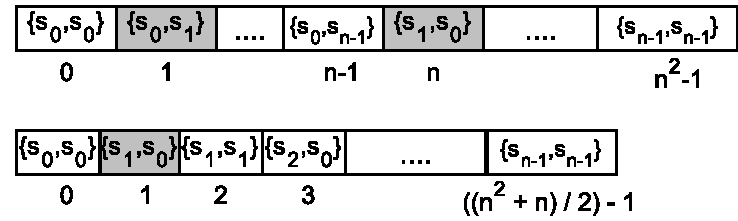
\includegraphics[width=\textwidth]{figs/memory.pdf}
	\caption{Indexing and placement of the state pair arrays. A simple placement of the pairs (on the left) uses redundant places for state pairs $\{s_i, s_j\}$, $i \neq j$, e.g., $\{s_1, s_2\}$ and $\{s_2, s_1\}$ in the figure. On the right, the indexing mechanism we used is shown.}
	\label{fig:mem}
\end{figure}

Due to architecture of GPU, algorithms that require less synchronization are more efficient. Since the number of threads is too high, creating frontier and remaining sets is an inefficient operation. Therefore we implemented S2R and S2F algorithms. For the CUDA version, each thread checks only one pair. To match pairs and threads, the above memory indexing formula is used.  Algorithm \ref{algo:find-min-parallel} uses constant number of threads. Each thread finds its local minimum, as in S2R and S2F. 
When a thread is done, it uses CUDA's {\tt atomicMin} operation to update the global minimum instead of sequential synchronization. 
